\documentclass[12pt]{article}
\usepackage[letterpaper, scale=0.85]{geometry} % Reduce document margins
\usepackage{graphicx}
\usepackage{amsmath}
\usepackage{amsfonts}
\usepackage{amssymb}
\usepackage{bm}
\usepackage{algorithm2e}

%opening
\setlength{\parindent}{0pt}

% Custome latex commands
\newcommand{\prob}[1]{\mathrm{Pr}\left(#1\right)}
\newcommand{\braces}[1]{\left\lbrace#1 \right\rbrace}

\begin{document}
\vspace{-1in}
\author{\bf Sta663 Final Project}
\title{\bf Stochastic Gradient Descent Hamiltonian Monte Carlo Applied to Bayesian Logistic Regression}
\date{Gilad Amitai and Beau Coker}
%\date{\today}
\maketitle 
%\thispagestyle{empty}


\begin{abstract}
	Hamiltonian Monte Carlo (HMC) is a Markov chain Monte Carlo algorithm for drawing samples from a probability distribution where proposed values are computed using Hamiltonian dynamics to find values of high acceptance probabilities. They allow us to explore sample states more efficiently than random walk proposals, but are limited by the expensive computation of the gradient of the potential energy function. Chen, Fox, and Guestrin propose the method Stochastic Gradient Hamiltonian Monte Carlo (SGHMC), a HMC algorithm that uses a subset of the data to compute the gradient. The authors find that the stochastic gradient is noisy and correct this with a friction term.

	In this project, we adapt the SGHMC to be used for Bayesian Logistic regression, implement this method in Python, optimize the code for computational efficiency, validate our approach using simulated data, and apply the algorithm to real world classification problems.
	
	Keywords: Hamiltonian Monte Carlo, Stochastic Gradient Hamiltonian Monte Carlo, Pima Indians Diabetes Dataset, Hockey Puck, Logistic Regression, Markov chain Monte Carlo
\end{abstract}

\section{Background}
Because this is a project about Hamiltonian Monte Carlo, imagine a frictionless puck on an icy surface of varying heights. The state of this puck is given by it's momentum $\bm{q}$ and position $\bm{p}$. The potential energy of the puck $U$ will be a function of only its height, while the kinetic energy will be a function of its momentum $K(q)=\frac{|\bm{q}|^2}{2m}$. If the ice is flat, the puck will move with a constant velocity. If the ice slopes upwards, the kinetic energy will decrease as the potential energy increases until it reaches zero, at which point it will slide back down. In the context of Bayesian statistics, we can think of the position of the puck as the posterior distribution we want to sample from, and the momentum variable are artificial constructs that allow us to efficiently move around our space. We propose samples from the Hamiltonian dynamics

\begin{gather*}
	d\theta=M^{-1}r\,dt\\
	dr = -\Delta U(\theta)\,dt
\end{gather*}

where $M$ is a mass function easily set to the identity matrix, and $U$ is the potential energy function given my $-\sum_{x\in\mathcal{D}}\log p(x|\theta)-\log p(\theta)$. To discretize time we implement the leapfrog method, which updates the momentum and position variables sequentially, first simulating the momentum variable over the interval $\frac{\epsilon}{2}$, then simulating the position variable over the entire learning rate $\epsilon$, and finally completing the simulation of the momentum variable over the time $\frac{\epsilon}{2}$.
\\

We can summarize the algorithm as follows:

\begin{algorithm}[H]
	\KwIn{Starting position $\theta^{(1)}$ and step size $\epsilon$.}
	\For{t=1, 2, \dots} {
		Sample momentum $r^{(1)}\sim\mathcal{N}(0, M)$\\
		$r_0=r_0+\frac{\epsilon}{2}\Delta U(\theta_0)$\\
		\For{i=1,\dots,m} {
			$\theta_i=\theta_{i-1}+\epsilon M^{-1}r_{i-1}$\\
			$r_i = r_{i-1} - \epsilon  \Delta U(\theta_i)$\\
		}
		$r_m = r_m -\frac{\epsilon}{2}\Delta U(\theta_m)$\\
		$(\hat{\theta}, \hat{r})=(\theta_m,r_m)$\\
		Sample $u\sim\mathrm{Uniform}[0, 1]$\\
		$\rho = \exp\braces{H(\hat{\theta}, \hat{r})-H(\theta^{(t)}, r^{(t)})}$\\
		\If{$u < \min(1, \rho)$}{$\theta^{(t+1)} = \hat{\theta}$}
	}
\end{algorithm}






\section{Description of Algorithm}
In their \textit{Stochastic Gradient Hamiltonian Monte Carlo}, Chen, Fox, and Guestrin propose using a subset $\tilde{\mathcal{D}}$ of the entire dataset $\mathcal{D}$ to compute
\begin{equation*}
	\Delta\tilde{U}(\theta)=-\frac{|\mathcal{D}|}{|\tilde{\mathcal{D}}|}\sum_{x\in\tilde{\mathcal{D}}}\Delta\log p(x|\theta) - \Delta\log p(\theta)
\end{equation*}
which can then be used in the Hamiltonian Monte Carlo equations in the stead of the gradient $\Delta U(\theta)$.

Logistic regression assigns the probability of success to a dichotomous response variable

\begin{equation*}
	\prob{y_i=1|\bm{x}_{i},\bm{\beta}}=\frac{\exp\braces{\bm{x}_i^T\bm{\beta}}}{1+\exp\braces{\bm{x}_i^T\bm{\beta}}}
\end{equation*}

where $\bm{x}_i$ is a vector of length $p$ covariates for data point $i$ and $\bm{\beta}$ is a vector of regression coefficients of length $p$. In a Bayesian framework, we would assign the a prior distribution on our unknown parameters $P(\bm{\beta})\sim\mathcal{N}(0, \sigma^2)$ where, for the purposes of our project, $\sigma^2$ is known. The corresponding posterior will be proportional to $P(\theta)\prod_{i=1}^n\prob{y_i|\bm{x}_i,\bm{\beta}}$, which would give us the potential energy function
\begin{equation*}
U(\bm{\beta})=-\log\left[P(\bm{\beta})\right] - \sum_{i=1}^n\log\left[\prob{y_i|\bm{x}_i,\bm{\beta}}\right]=\sum_{j=1}^p\frac{\beta_j^2}{2\sigma^2}-\sum_{i=1}^n\left[y_i(\bm{x}_i^T\bm{\beta})-\log(1+\exp\braces{\bm{x}_i^T\bm{\beta}})\right]
\end{equation*}
and gradient components
\begin{equation*}
\frac{\partial U}{\partial \beta_j}=\frac{\beta_j}{\sigma^2}-\sum_{i=1}^{n}x_{ij}\left[y_i-\frac{\exp\braces{\bm{x}_i^T\bm{\beta}}}{1+\exp\braces{\bm{x}_i^T\bm{\beta}}}\right]. 
\end{equation*}
In practice, the stochastic gradient is noisy since it is an approximation of the gradient. The paper suggests introducing a friction term to the momentum to dampen the movement of the chain. The algorithm will take a user specified friction term $C$ that is element-wise bigger than the noise model $B$. The noise model is unknown but can be set to zero for simplicity. The final algorithm will be:

\begin{algorithm}[H]
	\KwIn{Starting position $\theta^{(1)}$ and step size $\epsilon$.}
	\For{t=1, 2, \dots} {
		Sample momentum $r^{(1)}\sim\mathcal{N}(0, M)$\\
		\For{i=1,\dots,m} {
			$\theta_i=\theta_{i-1}+\epsilon M^{-1}r_{i-1}$\\
			$r_i = r_{i-1} + \epsilon \Delta\tilde{U}(\theta_i)-\epsilon C M^{-1}r_{i-1}+\mathcal{N}(0, 2(C-\hat{B})\epsilon)$\\
		}
		$(\theta^{t+1}, r^{t+1})=(\theta_m, r_m)$\\
	}
\end{algorithm}

\section{Optimization}
Any MCMC algorithm is inherently sequential, and so can't be parallelized (though multiple chains can be run at the same time). Each parameter's full conditional distribution depends on other parameters, so loops are a natural implementation. Unfortunately, loops are quite slow in Python. On the other hand, a compiled language has no such issues. In this section, we discuss an alternative, optimized version of our code that is written in C++ and is callable from Python via the Pybind11 package.

We feel this is a nice Both libraries are written with the same input syntax and function names, so they can be easily exchanged. A small difference is that the potential energy function and gradient function cannot be supplied by the user in the C++ implementation.\\

Note that one drawback to a C++ implementation is the limited availability of easy-to-use random sampling functions. To complete our algorithm, we wrote a random multivariate normal function based on a Cholesky decomposition (necessary for the momentum updates and noise terms) and a random sampling function (necessary for the stochastic gradient descent). Unfortunately, the random sampling function is quite slow, significantly dampening the impact from the low-level speedup.

To compare the performance of our two implementations, we make use of the {\tt %timeit} magic function. Unfortunately, while the {\tt %prun} profiler provides useful information on the Python implementation, it does not work on the Pybind11 implementation.
	
Starting with the stochastic gradient function, we see that...

Next, we see that the {\tt run_sghmc} function

As discussed, {\tt %prun} will not work for the Pybind11 version, so we can only examine the results for the unoptimized Python version.

\section{Application to Simulated Data}
To test our implementation of the algorithm, we simulated data with 50 covariates and 500 observations, where the covariates were sampled from a normal distribution with mean zero and variances 25, 5, and 0.4 sampled form a multinomial distribution with probability vector $(.05, .05, .9)$. Data was normalized to have mean zero and a standard deviation of one. No intercept was fit.\\

We can see that using the Hamiltonian Monte Carlo algorithm produced good mixing with energy decreasing downwards and converging:

\begin{figure}[H]
	\centering
	\begin{minipage}{0.45\textwidth}
		\centering
		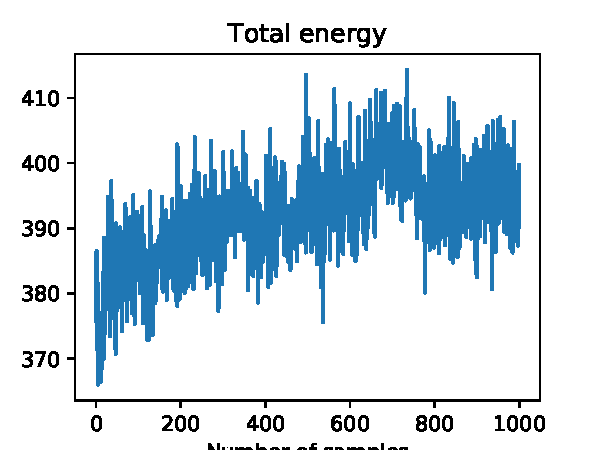
\includegraphics[width=0.9\textwidth]{hmc-energy-sim.pdf} % first figure 
	\end{minipage}\hfill
	\begin{minipage}{0.45\textwidth}
		\centering
		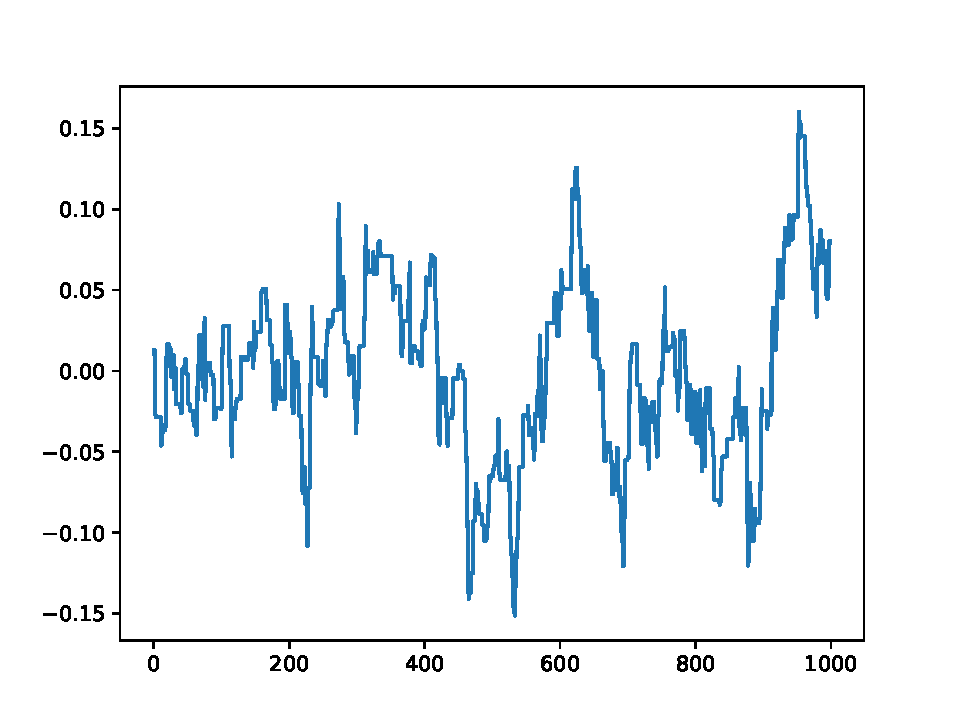
\includegraphics[width=0.9\textwidth]{hmc-trace-sim.pdf} % second figure 
	\end{minipage}
\end{figure}

We can see that using the Stochastic Gradient Hamiltonian Monte Carlo algorithm produced good mixing with energy decreasing downwards and converging:

\begin{figure}[H]
	\centering
	\begin{minipage}{0.45\textwidth}
		\centering
		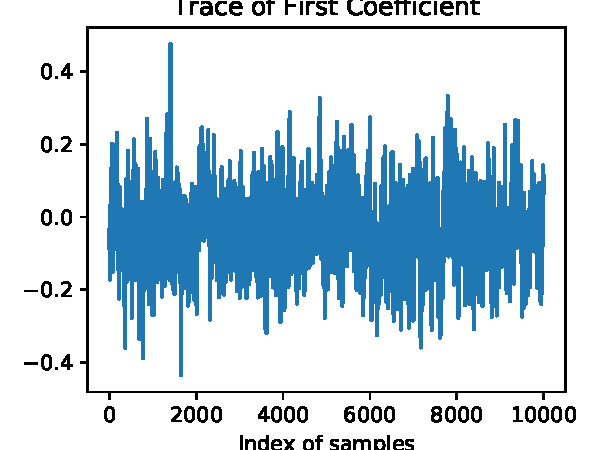
\includegraphics[width=0.9\textwidth]{sghmc-trace-sim.pdf} % first figure
	\end{minipage}\hfill
	\begin{minipage}{0.45\textwidth}
		\centering
		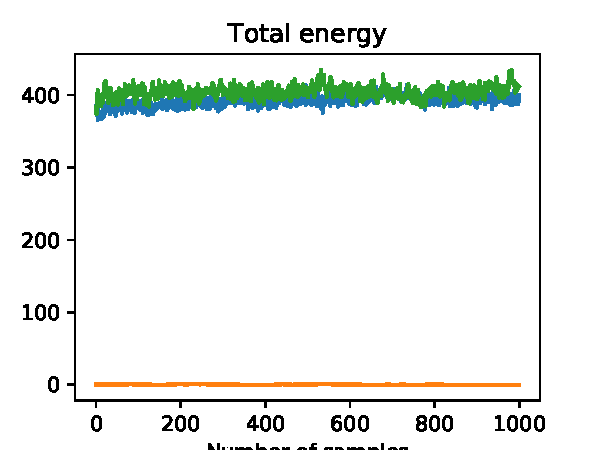
\includegraphics[width=0.9\textwidth]{sghmc-energy-sim.pdf} % second figure
	\end{minipage}
\end{figure}

We compared the coefficients produced by each algorithm to the MLE estimates to check for accuracy:

\begin{figure}[H]
	\centering
	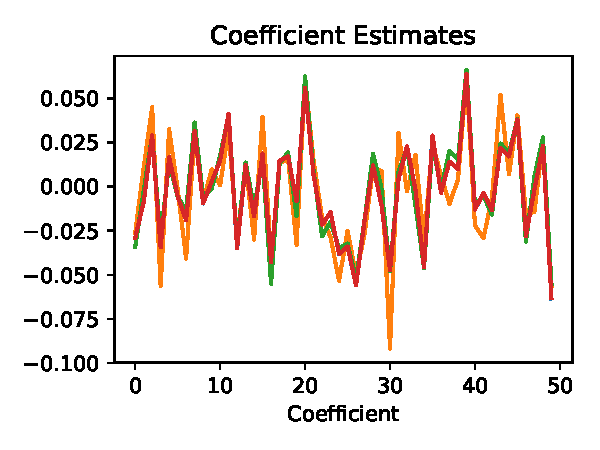
\includegraphics[width=0.45\textwidth]{coefs-sim.pdf}
\end{figure}

We see that all coefficients are fairly similar.

\section{Application to Real Data}
We used the Pima Indians Diabetes Dataset from the National Institute of Diabetes and Digestive and Kidney Diseases. This dataset has a binary response variable indicating if the sample has diabetes and eight covariates on 768 samples. The data was standardized to have mean zero and standard deviation one.\\



We can see that using the Hamiltonian Monte Carlo algorithm produced good mixing with energy decreasing downwards and converging:

\begin{figure}[H]
	\centering
	\begin{minipage}{0.45\textwidth}
		\centering
		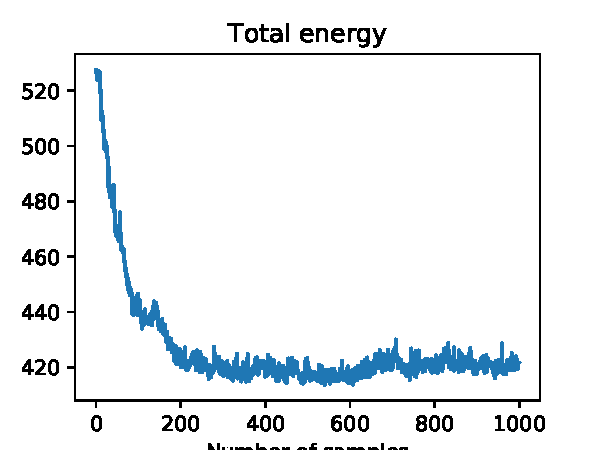
\includegraphics[width=0.9\textwidth]{hmc-energy-pima.pdf} % first figure itself
		\caption{first figure}
	\end{minipage}\hfill
	\begin{minipage}{0.45\textwidth}
		\centering
		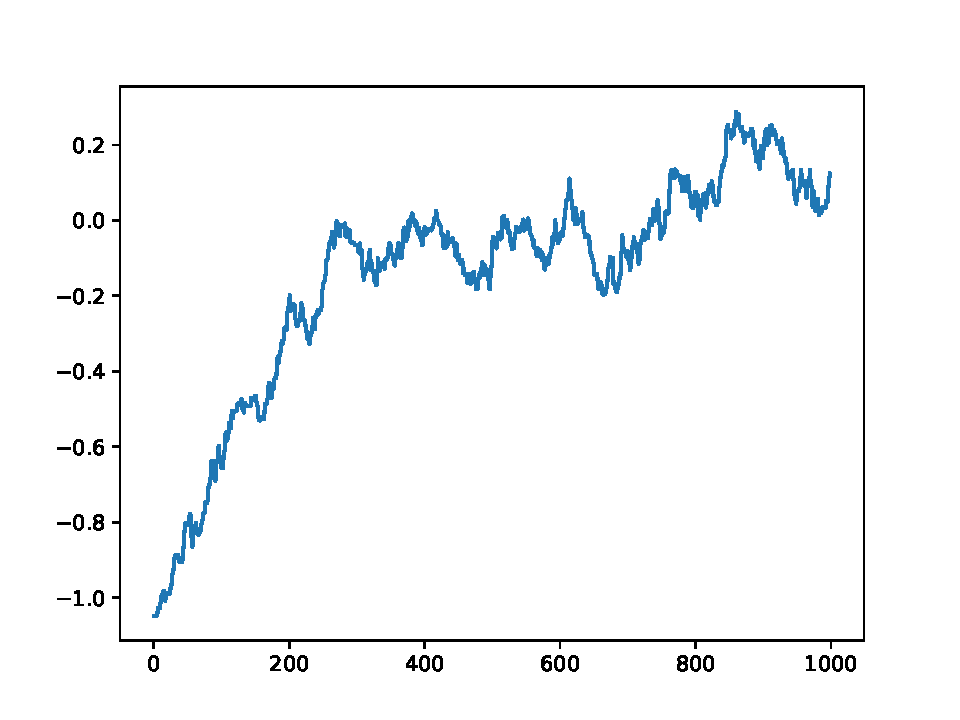
\includegraphics[width=0.9\textwidth]{hmc-trace-pima.pdf} % second figure itself
	\end{minipage}
\end{figure}

We can see that using the Stochastic Gradient Hamiltonian Monte Carlo algorithm produced good mixing with energy decreasing downwards and converging:

\begin{figure}[H]
	\centering
	\begin{minipage}{0.45\textwidth}
		\centering
		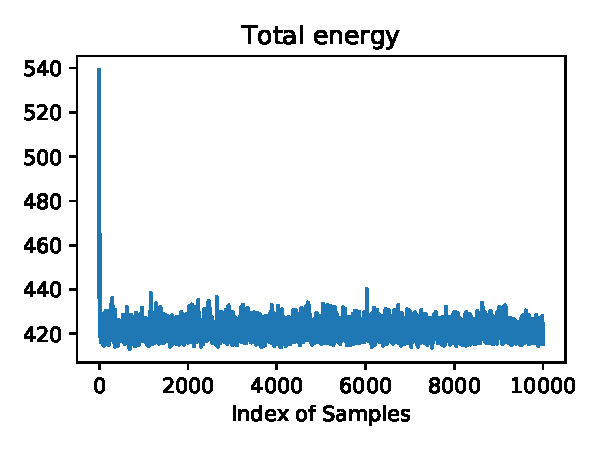
\includegraphics[width=0.9\textwidth]{sghmc-energy-pima.pdf} % first figure itself
		\caption{first figure}
	\end{minipage}\hfill
	\begin{minipage}{0.45\textwidth}
		\centering
		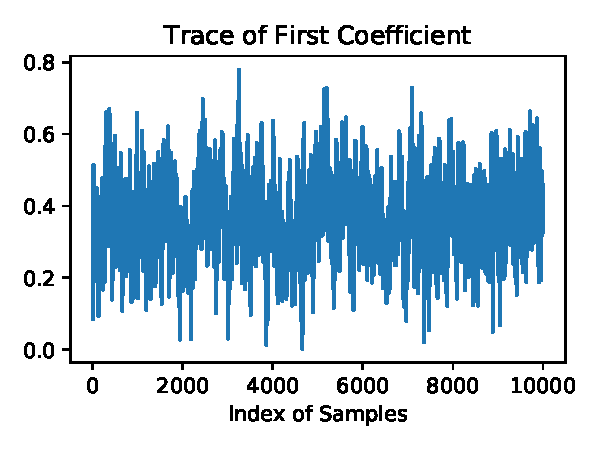
\includegraphics[width=0.9\textwidth]{sghmc-trace-pima.pdf} % second figure itself
	\end{minipage}
\end{figure}


We compared the coefficients produced by each algorithm to the MLE estimates to check for accuracy:

\begin{figure}[H]
	\centering
	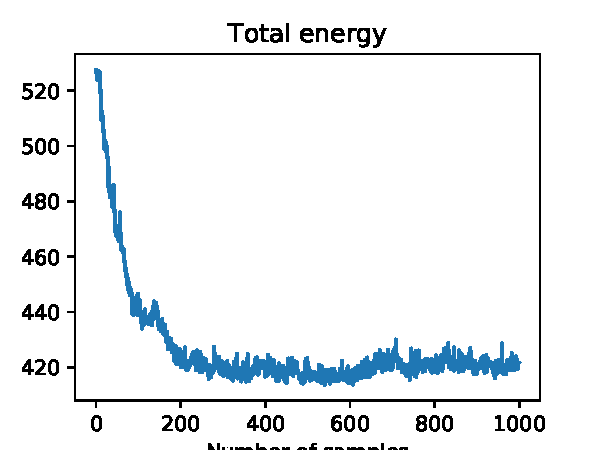
\includegraphics[width=0.45\textwidth]{hmc-energy-pima.pdf}
\end{figure}



\section{Comparative Analysis}
blah blah blah

\section{Discussion and Conclusion}
blah blah blah

\section{Bibliography}


\end{document}